%\usepackage{extsizes}
\documentclass[14pt, a4paper, russian]{report}

\linespread{1.3}

\usepackage{titlesec}
\usepackage[centertags]{amsmath}
\usepackage{amsthm,amsfonts,amssymb}
\usepackage{indentfirst}

\usepackage{extsizes}
\usepackage[left=25mm,right=10mm,top=20mm,bottom=20mm,bindingoffset=0cm]{geometry}

\usepackage{cmap}


% \usepackage{jmlda}
% \usepackage{amsmath}

\usepackage[T2A]{fontenc}
\usepackage[utf8]{inputenc}
\usepackage[english,russian]{babel}
%\usepackage{pscyr}
\RequirePackage{graphicx}
\RequirePackage{subfig}
\RequirePackage{pgfplots}
\usepackage{thmtools}   
\usepackage{hyperref}
\usepackage[nameinlink]{cleveref}


\newtheorem{lemma}{\indent Лемма}
\newtheorem{theorem}{\indent Теорема}
\newtheorem{corollary}{\indent Следствие}
\newtheorem{problem}{\indent Задача}
\newtheorem{remark}{\indent Замечание}
\newtheorem{definition}{\indent Определение}
\newtheorem{proposition}{\indent Утверждение}
\newtheorem{example}{\indent Пример}
\newtheorem{notation}{\indent Обозначение}

\crefname{lemma}{л.}{л.}
\crefname{theorem}{теор.}{теор.}
\crefname{corollary}{след.}{след.}
\crefname{definition}{опр.}{опр.}
\crefname{proposition}{утв.}{утв.}
\crefname{example}{прим.}{прим.}
\crefname{notation}{обозн.}{обозн.}


\newcommand{\order}[2]{#1_{(#2)}}

\newcommand{\T}{^{\text{\tiny\sffamily\upshape\mdseries T}}}

\graphicspath{{./img/}}


\def\XYtext(#1,#2)#3{\rlap{\kern#1\lower-#2\hbox{#3}}}

% Переопределение вставки графики
\newcounter{PictureNo}

\hyphenpenalty 100
\tolerance 10000


\newenvironment{Proof}%
    {\par\noindent{\bf Доказательство.}}%
    {\hfill$\scriptstyle\blacksquare$}

\usepackage{bbm}
\bibliographystyle{unsrt}

\addto\captionsenglish{\renewcommand{\figurename}{Рисунок}}

\addto\captionsenglish{\renewcommand{\proofname}{Доказательство}}

\makeatletter % эта строка НЕОБХОДИМА!
\renewcommand{\@chapapp}{Глава} 
\addto\captionsenglish{% Replace "english" with the language you use
  \renewcommand{\contentsname}%
    {Оглавление}%
}

\titleformat{\chapter}[display]
{\normalfont\bfseries\center}
{Глава \thechapter. }{0em}{}

\titleformat{\section}[block]
{\normalfont\bfseries\center}
{\thesection. }{0em}{}

\begin{document}
\begin{center}
\hfill \break
\footnotesize{Федеральное государственное автономное образовательное учреждение 
высшего образования}\\ 
\small{\textbf{<<Московский физико-технический институт (государственный университет)>>}}\\
\hfill \break
\normalsize{Факультет инноваций и высоких технологий}\\
\normalsize{Кафедра дискретной математики}\\
\end{center}
\footnotesize{\textbf{Направление подготовки:} 03.03.01 Прикладные математика и физика}\\
\hfill \break
\hfill \break
\hfill \break
\hfill \break
\begin{center}
\large{\textbf{Комбинаторные свойства обобщённых автоморфизмов Шакона}}\\
\normalsize{Бакалаврская работа}\\
\hfill \break
\hfill \break
\end{center}
 
\hfill \break
 
\begin{flushright}
\footnotesize{ 
\begin{tabular}{rl}
\textbf{Обучающийся:} & Слюсарев Владислав Владимирович \\
 & \underline{\hspace{3cm}} \\\\
\textbf{Научный руководитель:} & к. ф.-м. н., старший преподаватель\\
            & А. А. Приходько \\
 & \underline{\hspace{3cm}} \\\\
\end{tabular}
}
\end{flushright}

\hfill \break
\hfill \break
\hfill \break
\hfill \break
\hfill \break
\hfill \break
\begin{center} Москва 2018 \end{center}
\thispagestyle{empty} % выключаем отображение номера для этой страницы
 
% КОНЕЦ ТИТУЛЬНОГО ЛИСТА
 
\newpage

\tableofcontents{}

\chapter*{Введение}


Lorem ipsum dolor sit amet, consectetur adipiscing elit. Etiam mauris eros, venenatis id nisi ac, scelerisque dapibus metus. Aliquam scelerisque vulputate justo. Nunc ut commodo mauris. Etiam scelerisque sapien ac nisl euismod auctor. Sed eu commodo tortor, nec aliquam nulla. Nullam convallis, tellus sit amet porttitor vestibulum, orci metus sollicitudin mauris, at eleifend erat arcu et mauris. Donec vel tincidunt massa. Sed et consectetur neque. Integer libero eros, accumsan id congue ac, facilisis eu purus. Suspendisse potenti. Nullam blandit quis erat tempor ullamcorper. Suspendisse consequat condimentum turpis, et tempor lectus vulputate sed.

Nam in enim vel tortor congue cursus ac nec felis. Sed commodo arcu lorem, id gravida erat pulvinar id. Praesent maximus nisi ac ipsum malesuada tempus. Aliquam pellentesque in mi eu sagittis. Curabitur vitae quam risus. Ut sed erat auctor, pellentesque nulla eu, aliquam massa. Nunc laoreet enim velit, ut gravida odio tempus eget. Morbi nec congue libero, tincidunt vestibulum urna. Nulla sed lacus id arcu accumsan interdum. Suspendisse ut pharetra sem.

Aliquam erat volutpat. Etiam nec egestas velit. Curabitur eu metus ultricies magna cursus maximus. Proin nec eleifend ipsum. Nunc pulvinar nulla nisl, id finibus nunc faucibus eu. Cras libero magna, viverra eget eros non, fermentum tincidunt justo. Curabitur rhoncus felis lectus, ut tempus lectus congue at.

Sed tristique mauris a auctor egestas. Lorem ipsum dolor sit amet, consectetur adipiscing elit. Fusce accumsan aliquam porttitor. Fusce aliquam ante eu leo porttitor, vitae interdum dolor laoreet. Donec eget volutpat odio. Curabitur non massa tellus. Nullam in viverra mi, in hendrerit augue. Aenean vehicula dignissim elit, et condimentum mi facilisis eget. Interdum et malesuada fames ac ante ipsum primis in faucibus. Duis fermentum libero quis dapibus luctus. Sed eleifend ullamcorper sem, a tempor nunc consectetur eget. Curabitur ultrices posuere mollis. Donec iaculis leo id neque placerat, nec gravida sem venenatis. Nam elit augue, tristique vel rhoncus quis, aliquet dictum quam.

Aliquam risus sem, interdum vitae sodales sit amet, sollicitudin ut dui. Vivamus ut nisi congue, ultricies ante id, vehicula metus. Morbi eu sem id metus tincidunt tincidunt quis non libero. Vivamus at diam quis felis ullamcorper suscipit ac id turpis. In egestas id velit sit amet maximus. Sed a laoreet ligula, rhoncus ultrices dui. Integer nunc est, bibendum a consectetur eu, condimentum sit amet leo. Nulla facilisi. Nulla a ex ac mauris ultricies fermentum quis non tellus. Quisque lacinia sapien ac dui semper rutrum vitae ac velit. 

\newpage

\chapter{Основные определения}

\section{Основные обозначения и определения}

Пусть $p \ge 3$ --- произвольное натуральное число. Рассмотрим аддитивную группу вычетов $\mathbb{Z}_p$. 

\begin{definition}
Пространством $\Gamma$ назовём множество бесконечных последовательностей элементов из $\mathbb{Z}_p$:
$$\Gamma := \left\{x = \left(x_0, x_1, x_2, \ldots \right), x_k \in \{0, 1, \ldots, p - 1\} \right\}$$
Элементы $x_0, x_1, x_2, \ldots$ будем называть координатами элемента $x$.
\end{definition}
Далее мы также будем использовать множество 
$$\Gamma' := \Gamma \setminus \{(p-1,p-1,\ldots)\},$$
в котором каждая последовательность имеет в начале лишь конечное число элементов, равных $(p-1)$.

Отметим, что $\Gamma$ с операцией покоординатного сложения с переносом является компактной группой. Пусть $\lambda$ --- мера Хаара на группе $\Gamma$. Эта мера позволяет задать вероятностное пространство $(\Gamma, \mathcal{B}(\Gamma), \lambda)$.

\begin{notation} 
Пусть $a, b \in \mathbb{N},\ a \le b$ Множество $\{a, a+1, \ldots, b-1, b\} \subset \mathbb{N}$ будем называть отрезком и обозначать $\left[a, b\right]$. Учитывая естественное вложение $\mathbb{Z}_p$ в $\mathbb{N}$, мы будем использовать то же обозначение для соответствующего подмножества $\mathbb{Z}_p$, не оговаривая это особо в тех случаях, когда смысл данного обозначения читается однозначно.
\end{notation}

Относительно меры $\lambda$ все координаты $x_k, k \ge 0,$ являются независимыми одинаково распределёнными случайными величинами, имеющими дискретное равномерное распределение на множестве $\left[0, p-1\right]$. 

\begin{definition} Определим два преобразования, действующих на пространстве $\Gamma$ и сохраняющих меру $\lambda$:
\begin{itemize}
\item Преобразование сдвига на одну позицию влево $\sigma$: $x=\left(x_0, x_1, x_2, \ldots \right) \mapsto \sigma x = \left(x_1, x_2, \ldots \right)$
\item Преобразование <<прибавления единицы>> $S$: $x \mapsto x + 1$, где $1:=(1,0,0,\ldots) \in \Gamma'$, где сложение понимается в смысле групповой операции на $\Gamma$. 
\end{itemize}
\end{definition}
\begin{example}
Для иллюстрации действия этих преобразований зафиксируем $p=4$. 
\begin{itemize}
\item $\sigma (0,1,0,0,\ldots) = (1, 0, 0, \ldots)$
\item $S(1,0,0,\ldots) = (2,0,0,\ldots)$
\item $S(3,1,0,0,\ldots) = (0,2,0,0,\ldots)$
\item $S(3,3,3,2,1,1,\ldots)=(0,0,0,3,1,1,\ldots)$
\end{itemize}
\end{example}

Каждое целое число $j \ge 0$ можно отождествить с элементом множества $\Gamma'$: этот элемент получается при записи числа $j$ в системе счисления с основанием $p$ от младшего разряда к старшему с добавлением бесконечной последовательности нулей за последним знаком. Например, при $p=3$ мы отождествим число $42$ и элемент $(0,2,1,1,0,0,\ldots) \in \Gamma'$. Это обозначение согласовано с описанной выше операцией прибавления, так что мы можем говорить о прибавлении произвольного натурального числа к элементу $\Gamma'$: $S^j x = S(S(\ldots S(x)\ldots)) = x + j$ для любых $x \in \Gamma',\ j \ge 0$.

Преобразование $S^j$ является биективным для любого $j \ge 0$, поэтому мы можем говорить об обратном преобразовании $(S^j)^{-1} =: S^{-j}$. Аналогично предшествующему рассуждению, отождествим действие оператора $S^{-j}$ и вычитанию числа $j$: $S^{-j} x = x - j$.

\begin{definition}\label{phi}
Определим функционал $\phi: \Gamma' \to \mathbb{Z}$, возвращающий первую отличную от $(p-1)$ координату своего аргумента:
 \[\phi(x):=x_i\text{, если }x=(p-1, \ldots, p-1, x_i, x_{i+1}, \ldots)\]
\end{definition}
 Используя это определение, мы также определим семейство функционалов $\phi^{(m)}: \Gamma' \to \mathbb{Z},\ m \ge 0$:
\begin{definition}\label{phi_m}
    \[\phi^{(0)}(x):=0;\ \phi^{(m)}(x):=\phi(x)+\phi(Sx)+\ldots+\phi(S^{m-1}x)\]
\end{definition}
\begin{remark}
В определнии этих функционалов вычеты из $\mathbb{Z}_p$ естественным образом отождествляются с целыми числами. Таким образом, в определении $\phi^{(m)}(x)$ сложение осуществляется в множестве целых чисел, а не в группе вычетов.
\end{remark}

\begin{notation}
Пусть $n \ge 0$. Будем обозначать $\Delta_n := \sum\limits_{k=0}^{n}k = \frac{n(n+1)}{2}$. Положим также $\Delta_{-1} = 0$.
\end{notation}

\begin{example}\label{phi_delta}
Пусть $x = (x_0, x_1, \ldots) \in \Gamma'$ и $0 \le x_0 < p-1$. Если $0 < m \le p-1-x_0$, то $$\phi^{(m)}(x) = x_0 + (x_0 + 1) + \ldots + (x_0 + m - 1) = mx_0 + \Delta_{m-1}$$
Отметим, что при $m=0$ конечная формула также верна.
\end{example}

Заметим, что $\phi^{(m)}(x)$ является случайной величиной относительно пространства $(\Gamma, \mathcal{B}(\Gamma), \lambda)$, принимающей значения в $\mathbb{Z}$. Одним из основных объектов, рассматриваемых в настоящей работе, является эта случайная величина и её распределение $\pi_m$.
\begin{definition}\label{pi_m}
Пусть $j \in \mathbb{Z}$, тогда $\pi_m(j)=\lambda(\phi^{m}(x)=j)$ --- функция вероятности случайной величины $\phi^{(m)}$.
\end{definition}

При фиксированном $p$ распределения $\pi_m$ порождают семейство характеристических полиномов $P_m^p(t)$.

\begin{definition}\label{poly}
Зафиксируем натуральное число $p \ge 3$, тогда для любого целого $m \ge 0$ определим формальный полином $P_m^p(t):= \mathbb{E}_\lambda\left[ t^{\phi^{(m)}(x)}\right] = \sum\limits_{j=0}^m \pi_m(j) t^j$.
\end{definition}

Данные полиномы, рассматриваемые как семейство с параметром $m$ при фиксированном $p$, являются центральным предметом изучения в настоящей работе.

\section{Обобщённый автоморфизм Шакона}

Зафиксируем произвольное $p \ge 3$. Определим последовательность высот $\{h_n\}_{n \ge 0}$ при помощи рекуррентного соотношения:
$$\begin{cases}
h_0 = 1 \\
h_n = p h_{n-1}+\Delta_{p-2},& n > 0 
\end{cases}$$

Для каждого $n \ge 0$ определим пространство
$$X_n:=\{(x,i): x \in \Gamma',\ 0 \le i \le h_{n-1} + \phi(x)\}$$

Рассмотрим преобразование $T_n$ пространства $X_n$, определяемое по правилу
$$T_n(x, i) := \begin{cases}
(x,i+1), & \text{ если } i+1 \le h_n - 1 + \phi(x) \\
(Sx,0), & \text{ если } i=h_n-1+\phi(x). \end{cases}$$

Также определим биективное отображение $\psi_n : X_n \mapsto X_n+1$:
$$\psi_n(x,i):=(\sigma x, x_0 h_n + i + \mathbb{1}\{x_0=p-1\})$$

Отметим, что $\psi_n$ сопрягает преобразования $T_n$ и
$T_{n+1}$.

Введём вероятностную меру $\mu_n$ на пространстве $X_n$: для фиксированного $i$ и подмножества
$A \subset \{(x, i), x\in\Gamma' \}$ положим
$$\mu_n(A):=\frac{1}{h_n + \Delta_{p-2}/2} \lambda (\{x \in \Gamma', (x, i) \in A\}).$$
% WRONG, NOT 1/2 BUT MEAN OMEGA

Преобразование $T_n$ сохраняет меру $\mu_n$, а отображение $\psi_n$ устанавливает соответствие между $\mu_n$ и $\mu_{n+1}$. Таким образом, все динамические системы $(X_n, T_n, \mu_n)$ изоморфны.

Для каждого $ 0 \le i \le h_{n-1}$ определим множество
$E_{n,i} := \{(x, i) : x \in \Gamma'\} \subset X_n$. Имеем $E_{n,i} = T^i_n E_{n,0}$. Последовательность
 $$\{E_{n,0},\ldots,E_{n,h_n-1}\}$$
называется башней Рохлина высоты $h_n$ для преобразования $T_n$ \cite{rokhlin_towers}. Кроме того, для любых $n \ge 0$ и $0 \le i \le h_n-1$ верно 
\begin{equation}\label{eq:embedding}
(En,i) = E_{n+1,i} \sqcup E_{n+1,h_n+i} \sqcup E_{n+1,2h_n+i+1}.
\end{equation}

Таким образом, мы построили цепочку вложенных башен, которая определяет сохраняющее меру преобразование $T$. Если $p=3$, описанная процедура буквально задаёт классический автоморфизм Шакона: этот случай разобран в работе \cite{weaklimits}. Для любого $p > 3$ получается похожее преобразование, которое будем называть \emph{обобщённым автоморфизмом Шакона}. В данной работе мы исследуем свойства обощённого автоморфизма Шакона и сравним его свойства с классическим случаем.

\chapter{Палиндромическое свойство характеристических полиномов}
Одним из важных свойств, доказанных для классического автоморфизма Шакона, является симметрия коэффициентов его характеристических полиномов. Для классического случая $p=3$  это свойство доказано в работе \cite{weaklimits}. Покажем, что в общем случае $p \ge 3$ оно также выполнено.

Дадим формальное определение доказываемого свойства. Для этого рассмотрим более широкий класс функционалов, подобных определённому в \cref{phi} функционалу $\phi$.
\begin{definition} \label{psi}
Пусть $\omega: \mathbb{Z}_p \setminus \{p-1\} \to \mathbb{Z}$ - некоторая функция. Тогда будем говорить, что функционал $\psi: \Gamma' \to \mathbb{Z}$ задаётся функцией $\omega$, если
$$
    \psi(x) = \begin{cases}
                    \omega(x_0),x_0 \in \left[0,  p - 2\right] \\
                    \phi(\sigma x), & x_0 = p - 1
                \end{cases}
$$

Для заданного $\psi$ определим функционал $\psi^{(m)}$ аналогично \cref{phi_m} и функцию вероятности $\pi_m[\psi]$ аналогично \cref{pi_m}
\end{definition}

В соответствии с этим определением функционал $\phi$ задан тождественной функцией $\omega(j)=j$. Отметим, что в случае $p=3$ это единственный (с точностью до биекции, которая, как будет показано далее, не влияет на свойства коэффициентов) нетривиальный функционал. 

Определим палиндромическое свойство для функционала $\psi$, заданного произвольной функцией $\omega$.

\begin{definition}\label{palindromic}
Пусть $\psi$ --- функционал, заданный функцией $\omega$, обозначим $\omega_\star = \min\limits_x \omega(x),\ \omega^\star = \max\limits_x \omega(x), \delta=\omega^\star - \omega_\star$. Будем говорить, что  $\psi$  \emph{обладает палиндромическим свойством} тогда и только тогда, когда
$$
\forall j,\ 0 \le j \le m\delta:   \pi_m[\psi](m\omega_\star + j)=\pi_m[\psi](m\omega^\star-j)
$$
\end{definition}

В \cref{poly} для каждого $j$ значение функции вероятности $\pi_m(j)$ является коэффициентом при $t^j$ в полиноме $P_m^p(t)$, а значения $m\omega_\star$ и $m\omega^\star$. Поэтому данное определение задаёт нужный вид полиномов: коэффициенты при мономах в канонической записи читаются <<справа налево>> и <<слева направо>> одинаково.

Задача доказательства симметрии коэффициентов сводится к поиску достаточного условия для палиндромичности функционала $\psi$. Получив это достаточное условие, мы покажем, что оно выполнено для $\phi$.

\begin{definition}\label{antipalindromic}
Функцию $\omega$ назовём \emph{антипалиндромической}, если
\[\begin{cases}
	\mathrm{Ran }\ \omega = \left[0, \zeta\right], \text{где } \zeta := p-2 \\
	\forall j,\ 0 \le j \le p-2: \  \omega(j) = \zeta - \omega(p-2-j)
\end{cases}\]
\end{definition}
\begin{remark}
Здесь мы накладываем сильное условие на $\omega$: мы требуем, чтобы её значения заполняли отрезок. Фактически, это нужно лишь для простоты последующих рассуждений: впоследствии от него можно будет отказаться, получив соответствующее обобщение свойств антипалиндромических функций.
\end{remark}


\begin{example} \label{classic_omega}
Функция $\omega(j)=j$ является антипалиндромической для любого $p$. Действительно,
$$
\mathrm{Ran }\ \omega = \left[0, p-2\right]
$$
$$
\omega(j) = j = p-2 - (p-2-j) = p-2 - \omega(p-2-j)]
$$
\end{example}

\begin{figure}[!h]
    \subfloat[$\omega(j)=j$]{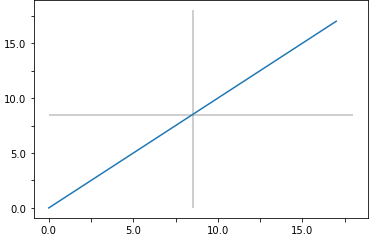
\includegraphics[width=0.5\linewidth]{linear}}
    \subfloat[$\omega(x)=((\frac{x+1}{p}) + 1)/2$]{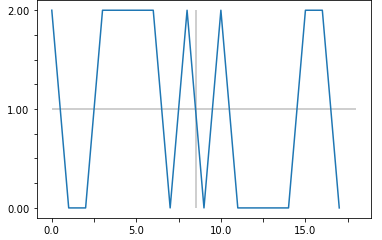
\includegraphics[width=0.5\linewidth]{legendre}}\\
    \caption{\small Примеры антипалиндромических функций для $p=19$}
\label{fig:antipalindromic}
\end{figure}

На \cref{fig:antipalindromic} показаны графики двух антипалиндромических функций. Для первой из них --- линейный функции $\omega(x)=x$ --- это свойство доказано выше. Вторая порождена символом Лежандра $(\frac{x+1}{p})$, её антипалиндромичность для простых чисел $p$ вида $4k+3$ является выражением свойства символа Лежандра и следует из закона квадратичной взаимности \cite{vinogradov}.

Следующая теорема даёт простейшее достаточное условие палиндромичности.

\begin{theorem}\label{palindromic_theorem}
Если функция $\omega$ антипалиндромическая, то заданный ей функционал $\psi$ обладает палиндромическим свойством.
\end{theorem}

Для доказательства теоремы понадобится следующая лемма:

\begin{lemma}\label{antipalindromic_lemma}
Пусть функционал $\psi$ задан антипалиндромической функцией. Тогда случайные последовательности $\{\psi(S^j x)\}_{j \ge 0}$ и $\{ \zeta - \psi(S^{-j} x)\}_{j \ge 0}$ равны по распределению. 
\end{lemma}
\begin{proof}
Прежде чем доказать лемму, приведём способ вычисления элементов данной последовательности.

Пусть $x \in \Gamma \setminus \{(p-1,p-1,\ldots)\}$ --- произвольный элемент. Определим порядок элемента $x$ как индекс его первой отличной от $p-1$ координаты: $\mathrm{order}(x) = k \ge 0$, если  $x_0=x_1=\ldots=x_{k-1}=p-1$ и $x_k \ne p-1$.

Рассмотрим последовательность $(\ldots, x-1,x,x+1, \ldots)$.  Легко видеть, что последовательность первых координат $(\ldots, (x-1)_0,x_0,(x+1)_0, \ldots)$ является периодической: в ней повторяется набор
$(0, 1, 2, \ldots,p-2, p-1$. Отсюда видно, что в исходной последовательности элементы порядка $0$ встречаются группами по $p-2$ элемента, между которыми находится ровно один элемент более высокого порядка (его первая координата $p-1$). Таким образом, последовательность
$\{\psi(S^j x)\}_{j \ge 0}$ состоит из блоков $\omega(0),\omega(1),\ldots, \omega(p-2)$, разделяемых одним элементом --- образом точки более высокого порядка. Чтобы найти недостающие элементы с индексами $j$, для которых $\mathrm{order}(S^j x) \ge 1$, отметим следующий факт. Если $x$ начинается с $p-1$, то для всех $j \ge 0$ выполнено $\psi(x+pj)=\psi(\sigma x + j)$. Следовательно, недостающие элементы последовательности соответствуют значениям $\{\psi(S^j \sigma x)\}_{j \ge 0}$. В свою очередь, для них верны приведённые выше рассуждения о последовательности первых координат: оказалось, что подпоследовательность с индексами, соответствующими элементам порядка $1$ и выше, повторяет всю исходную последовательность: она как бы вложена сама в себя.

Таким образом, мы можем построить всю последовательность $\{\psi(S^j x)\}_{j \ge 0}$ рекурсивно:
\begin{enumerate}
\item Выписываем значения для элементов порядка $0$ блоками $\omega(0),\omega(1),\ldots, \omega(p-2)$, разделяя их пропусками в один элемент. Мы выполняем циклический сдвиг блоков так, чтобы последовательность начиналась с $\omega(x_0)$, если $x$ --- элемент нулевого порядка, и с пропуска иначе.
\item Заполняем пропуски. Для этого рекурсивно запускаем процедуру для $x' = \sigma x$ и вписываем полученные элементы последовательно на места пропусков.

\begin{figure}[!h]
{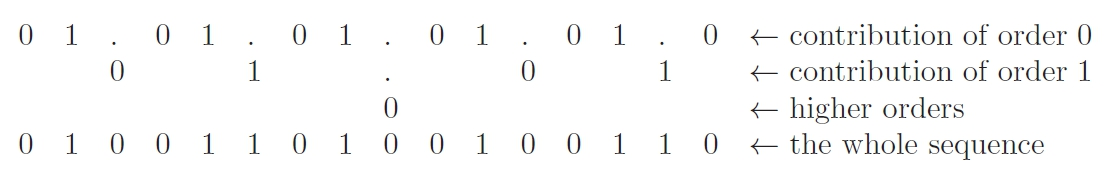
\includegraphics[width=\linewidth]{recursion}}
    \caption{\small Пример построения последовательности $\{\psi(S^j x)\}$ для  $p=3$ и $x=0$ \cite{weaklimits}}
\label{fig:antipalindromic}
\end{figure}

\end{enumerate}

Перейдём к доказательству леммы. 

Заметим, что последовательность $\{ \zeta - \psi(S^{-j} x)\}_{j \ge 0}$ можно получить из $\{\psi(S^j x)\}_{j \ge 0}$ композицией двух сохраняющих меру преобразований:
\begin{enumerate}
\item Преобразование <<обращения>>  $\{a_j\}_{j \ge 0} \mapsto \{a_{-j}\}_{j \ge 0}$ 
\item Преобразование <<поэлементного дополнения>>, заменяющее каждый элемент $k \in \{b_j\}_{j \ge 0}$ на  $\zeta-k$; таким образом, получается последовательность $\{ \zeta - b_j\}_{j \ge 0}$ .
\end{enumerate}
По определению антипалиндромических функций, такое преобразование является тождественным для подпоследовательности элементов порядка $0$. В силу описанной выше конструкции, оно является тождественным для всей последовательности $\{\psi(S^j x)\}_{j \ge 0}$. Поскольку преобразование биективно и сохраняет меру, эти последовательности равны по распределению, что и требовалось доказать.
\bigskip\\
\end{proof}

Перейдём к доказательству теоремы.
\begin{proof}
В \cref{psi} подставим $\psi_\star = 0, \psi^\star = \delta = \zeta$. Достаточно показать, что  \[\forall j,\ 0 \le j \le m\zeta: \pi_m[\psi](j) = \pi_m[\psi](m \zeta - j).\]
Действительно,
$$\pi_m[\psi](m \zeta - j) = \lambda(\psi^{(m)}(x)=m\zeta-j)=$$ 
$$=\sum\limits_{(\psi_1, \ldots, \psi_m)} \lambda\big(\psi(x)=\psi_1, \psi^{(2)}(x) = \psi_2, \ldots, \psi^{(m)}(x)=\psi_m\big) \mathbb{I} (\psi_1 + \ldots + \psi_k = m\zeta - j) =$$
$$ = \sum\limits_{(\psi_1, \ldots, \psi_m)} \lambda\big(\psi(x)=\psi_1, \psi^{(2)}(x) = \psi_2, \ldots, \psi^{(m)}(x)=\psi_m\big) \mathbb{I} \big((\zeta-\psi_1) + \ldots + (\zeta-\psi_m) = j\big)$$
По предыдущей лемме это равно
$$\sum\limits_{(\psi_1, \ldots, \psi_m)} \lambda\big(\psi(x)=\zeta-\psi_m, \psi^{(2)}(x) = \zeta-\psi_{m-1}, \ldots, \psi^{(m)}(x)=\zeta-\psi_1\big) \mathbb{I} \big(\sum\limits_k (\zeta-\psi_k) = j\big) = \left< \psi_k := \zeta - \psi_k \right> =$$
$$ =\sum\limits_{(\psi_1, \ldots, \psi_m)} \lambda(\psi(x)=\psi_1, \psi^{(2)}(x) = \psi_2, \ldots, \psi^{(m)}(x)=\psi_m) \mathbb{I} (\psi_1 + \ldots + \psi_m = j) =  \lambda(\psi^{(m)}(x)=j)= $$
$$ =\pi_m[\psi](j)$$
\end{proof}

Результат этой теоремы может быть обобщён на более широкий класс функций. Фактически, мы сможем отказаться от ограничения на область значений функции $\omega$ в \cref{antipalindromic}.

\begin{corollary}
Коэффициенты характеристических полиномов обобщённого автоморфизма Шакона симметричны для любого $p \ge 3$ .
\end{corollary}
\begin{proof}
Отметим, что в соответствии с \cref{poly} коэффициентами полинома $P_m^p(t)$ являются значения $\pi_m(t)$. В силу \cref{palindromic} требование симметрии коэффициентов --- в точности то же самое, что палиндромическое свойство для $\phi$. В \cref{classic_omega} показали, что $\phi$ удовлетворяет условию \cref{palindromic_theorem}, и, следовательно, обладает палиндромическим свойством.
\end{proof}

Отдельный познавательный интерес представляет описание как можно более широкого класса функций, порождающих функционалы с палиндромическим свойством. Докажем несколько утверждений, обобщающих результат теоремы.

\begin{corollary}[Об аффинном преобразовании]
Пусть $\omega:[0,p-2] \rightarrow [0, \zeta]$ --- антипалиндромическая функция, тогда для любых $a > 0, b \ge 0$ функционал, заданный по правилу
$$\psi'(x) = \begin{cases}
                    a \omega(x_0) + b, & 0 \le x_0 \le p - 2 \\
                    \psi'(\sigma x), & x_0 = p - 1
                \end{cases}$$
обладает палиндромическим свойством.
\end{corollary}
\begin{proof}
Пусть $\pi_m'(j) = \lambda(\psi'^{(m)}(x)=j)$. В терминах \cref{antipalindromic}, $\psi_\star = b, \psi^\star = a\zeta + b, \delta = a\zeta$. Покажем, что $\pi_m'(mb + j) = \pi_m' (m(a\zeta+b)-j)$.

Выполним деление с остатком: $j = qa + r$. По построению $\psi'$ верно, что $\pi_m'(mb + qa + r) = 0$, если $r \ne 0$. Кроме того, $m(a\zeta+b)-j = m(a\zeta+b)-qa - r = mb + (m\zeta -q)a - r$, и следовательно, $\pi_m' (m(a\zeta+b)-j) = 0$, если $r \ne 0$.\\
Таким образом, достаточно показать, что $\pi_m'(mb + qa) = \pi_m' (m(a\zeta+b)-qa)$.
Заметим, что значения $\psi$, заданной функцией $\omega$, возможно восстановить из значений $\psi'$. Действительно, рассмотрим биекцию $i: \{b, a + b, 2a + b \ldots, a\zeta + b\} \rightarrow [0, \zeta]$, такую, что $i(j) = \frac{j-b}{a}$. Легко видеть, что $i(\psi'(x))=\psi(x)$. Аналогично, определим $i^{(m)}(j) = \frac{j-mb}{m}$ и получим $i^{(m)}(\psi'^{(m)}(x))=\psi(x)$. Отображение $i^{(m)}$ также является биекцией.

Теперь докажем, что $\pi_m'(mb + qa) = \pi_m' (m(a\zeta+b)-qa)$, пользуясь биективностью $i^{(m)}$.

\[\pi_m'(mb + qa) = \lambda(\psi'^{(m)}(x)=mb + qa) = \lambda\big(i^{(m)}(\psi'^{(m)}(x))=i^{(m)}(mb + qa)\big)  =\]\[= \lambda(\psi^{(m)}(x)= \frac{mb-qa-mb}{m})= \lambda(\psi^{(m)}(x)= q)=\pi_m(q)\]
Аналогично, $\pi_m' (m(a\zeta+b)-qa) = \pi_m(m\zeta - q)$. Так как $\omega$ --- антипалиндромическая функция, по \cref{palindromic_theorem} $\pi_m(q) = \pi_m(m \zeta - q)$, и следовательно $\pi_m'(mb + qa) = \pi_m' (m(a\zeta+b)-qa)$.
\end{proof}

Благодаря этому следствию мы можем показывать палиндромичность для достаточно большого класса функций. В частности, из этого следует, что если значения $\omega$ образуют арифметическую прогрессию, то она порождает палиндромический функционал. Действительно, любая такая функция получается аффинным преобразованием из антипалиндромической.

Отметим, что при доказательстве этого следствия мы не пользовались свойствами аффинного преобразования как такового. Фактически, оно является частным случаем более общего факта:
\begin{corollary}{О сохранении палиндромического свойства}
Пусть $\psi$ обладает палиндромическим свойством, и пусть функционал $\psi'$ таков, что для любого $m \in \mathbb{N}$ существует биекция $$i^{(m)}: \mathrm{Ran}\ \psi'^{(m)} \rightarrow \mathrm {Ran}\ \psi^{(m)}.$$ Тогда $\psi'$ также обладает палиндромическим свойством.
\end{corollary}
Доказательство в точности повторяет рассуждения из предыдущей леммы. Важно, что рассматриваемая здесь биекция --- не просто соответствие значений $\omega$. Взаимная однозначность должна сохраняться для всех порядков $m$ функционала $\phi$, и это требование нельзя ослабить. В частности, преобразование $\omega(j) \mapsto \omega^2(j)$ является биекцией, но не сохраняет палиндромического свойства для задаваемых функционалов.

\chapter{Рекуррентные соотношения для характеристических полиномов}

В этой главе мы выведем рекуррентные соотношения, которые позволят построить всё семейство характеристических полиномов алгебраически.

Для начала докажем простую лемму.

\begin{lemma}\label{simple_case} $P_{pm}^p(t)=t^{m\Delta_{p-2}}P_m^p(t)$
\end{lemma}
\begin{proof}
Пусть $x \in \Gamma'$. В соответствии с конструкцией для последовательности $\{\phi(S^j x)\}_{j \ge 0}$ (см. доказательство \cref{antipalindromic_lemma}), мы можем представить значение $\phi^{(pm)}(x)$ как сумму по порядкам аргумента: 
$$ \phi^{(pm)}(x) = \sum\limits_{\mathrm{order}(S^j x) = 0}^{0 \le j \le pm-1}\phi(S^j x) + \sum\limits_{\mathrm{order}(S^j x) \ge 1}^{0 \le j \le pm-1} \phi(S^j x)$$
\begin{itemize}
\item Найдём вклад в сумму элементов порядка $0$. Этих элементов ровно $(p-1)m$. Значения $phi$ на этих элементах вычисляются непосредственно по первой координате, так что они образуют периодическую последовательность $\ldots,(p-2),0,1,2,...,(p-2),0,1,\ldots$ Таким образом, сумма по элементам порядка $0$ распадается на $m$ одинаковых блоков, в каждом из которых встречаются по одному разу все числа отрезка $\left[ 0, p-2 \right]$. Их сумма равна $\Delta_{p-2}$, так что полный вклад элементов порядка $0$ составляет $\frac{(p-1)(p-2)}{2}m=m\Delta_{p-2}$
\item В соответствии с конструкцией из \cref{antipalindromic_lemma}, сумма по элементам порядка $1$ и выше в точности равна $\phi^{(m)}(\sigma x)$.
\end{itemize}
Итак, $\phi^{pm}(x) = m\Delta_{p-2} + \phi^{(m)}(\sigma x)$. По определению полиномов $P_m^p(t)$ отсюда следует 
$$P_{pm}^p(t) = \mathbb{E}_\lambda\left[ t^{\phi^{(pm)}(x)}\right] = 
\mathbb{E}_\lambda\left[ t^{m\Delta_{p-2} + \phi^{(m)}(\sigma x)}\right] = 
t^{m\Delta_{p-2}} \mathbb{E}_\lambda \left[ t^{\phi^{(m)} (\sigma x)}  \right] = 
t^{m\Delta_{p-2} }P_m(t)$$
\end{proof}



\chapter{Моделирование данных и статистик}

Покажем на экспериментальных примерах, что статистика $\hat{a}$ имеет основания быть состоятельной и асимпотически нормальной. Для этого расмотрим следующие примеры распределений:
\begin{enumerate}
  \item $X_l \sim \mathcal{N}(10, 1)$, параметр сдвига $a = 10$ (рис. \textit{fig:normshift}).
  \item $X_l \sim Exp(1)$ с параметром сдвига $a = 5$ (рис. \textit{fig:expshift}).
\end{enumerate}
В ходе каждого эксперимента, сгенерируем 1000 выборок размера $n = 1000000$, зададим величину $1 \le k_n \le 1000 = \sqrt{n}$, и рассмотрим графики поведения среднего значения статистики $\hat{a}_{\max}$ в зависимости от $k$, гистограммы поведения статистики при $k = 1000$.

%\begin{figure}[!h]
%    \subfloat[Гистограмма]{\includegraphics[width=0.5\textwidth]{./norm_hist_shift.eps}}
%    \subfloat[Значение $\hat{a}_{\max}$]{\includegraphics[width=0.5\textwidth]{./norm_mean_shift.eps}}\\
%    \caption{\small Данные по выборке из нормального распределения, параметр сдвига $a = 10$}
%    \label{fig:norm_shift}
%\end{figure}

%\begin{figure}[!h]
 %   \subfloat[Гистограмма]{\includegraphics[width=0.5\textwidth]{./exp_hist_shift.eps}}
%    \subfloat[Значение $\hat{a}_{\max}$]{\includegraphics[width=0.5\textwidth]{./exp_mean_shift.eps}}\\
%    \caption{\small Данные по выборке из экспоненциального распределения, параметр сдвига $a = 5$}
%    \label{fig:exp_shift}
%\end{figure}


Из представленных графиков видно, что в рассмотренных распределениях гистограмма похожа на график плотности нормального распределения, а среднее значение сходится к истинному значению параметра, поэтому статистика $\hat{a}_{\max}$ может быть подвергнута дальнейшему исследованию.



Аналогично предыдущему случаю, построим графики и гистограммы для следующих распределений:

\begin{enumerate}
  \item $X_l \sim \mathcal{N}(5, 25)$, параметр масштаба $b = 5$,
  \item $X_l \sim Exp(10)$ с параметром масштаба $b = 10$,
  \item $X_l \sim Pareto(1.2)$, параметр масштаба $b = 10$.
\end{enumerate}


%\begin{figure}[!h]
%    \subfloat[Гистограмма]{\includegraphics[width=0.5\textwidth]{./norm_hist_scale.eps}}
%    \subfloat[Значение $\hat{b}_{\max}$]{\includegraphics[width=0.5\textwidth]{./norm_mean_scale.eps}}\\
%    \caption{\small Данные по выборке из нормального распределения, параметр $b = 5$}
%    \label{fig:norm_scale}
%\end{figure}

%\begin{figure}[!h]
%    \subfloat[Гистограмма]{\includegraphics[width=0.5\textwidth]{./exp_hist_scale.eps}}
%    \subfloat[Значение $\hat{b}_{\max}$]{\includegraphics[width=0.5\textwidth]{./exp_mean_scale.eps}}\\
%    \caption{\small Данные по выборке из экспоненциального распределения, параметр $b = 10$}
%    \label{fig:norm_scale}
%\end{figure}


%\begin{figure}[!h]
%    \subfloat[Гистограмма]{\includegraphics[width=0.5\textwidth]{./pareto_hist.eps}}
%    \subfloat[Значение $\hat{b}_{\max}$]{\includegraphics[width=0.5\textwidth]{./pareto_mean.eps}}\\
%    \caption{\small Данные по выборке из распределения Парето, параметр $b = 10$}
%    \label{fig:pareto_scale}
%\end{figure}


Как и в предыдущем случае, гистограммы оценок параметра масштаба для $k = 1000$ похожи на гистограммы плотности нормального распределения.

\newpage
\bibliography{chacon}


\end{document}
